\section{Results}\label{sec:results}

\subsection{Dataset Characteristics}

Our analysis utilized 702 real embryo samples with quality scores ranging from 0.004 to 0.999 (mean: 0.592 ± 0.287). The binary classification distribution showed 66.7\% positive blastulation outcomes (468 successful, 234 unsuccessful), reflecting typical clinical IVF success rates and confirming the dataset's clinical representativeness.

\subsection{Parametric Cycle Prediction Calculator Performance}

The parametric calculator successfully demonstrated comprehensive IVF cycle simulation capabilities, providing transparent relationships between patient-specific factors and predicted outcomes throughout the entire treatment process from oocyte retrieval to live birth, with clinically interpretable counseling tools.

\subsubsection{AMH-Based Predictions}

Figure~\ref{fig:calculator_amh} illustrates oocyte yield predictions across AMH levels and age groups. The model captures the expected relationship where higher AMH values consistently predict better retrieval outcomes, with the effect being most pronounced in younger patients. Importantly, the visualization avoids misleading fixed AMH reference ranges, instead emphasizing the age-dependent nature of AMH interpretation through updated annotations clarifying effects "at any given age" and "at any given AMH level."

\begin{figure}[H]
    \centering
    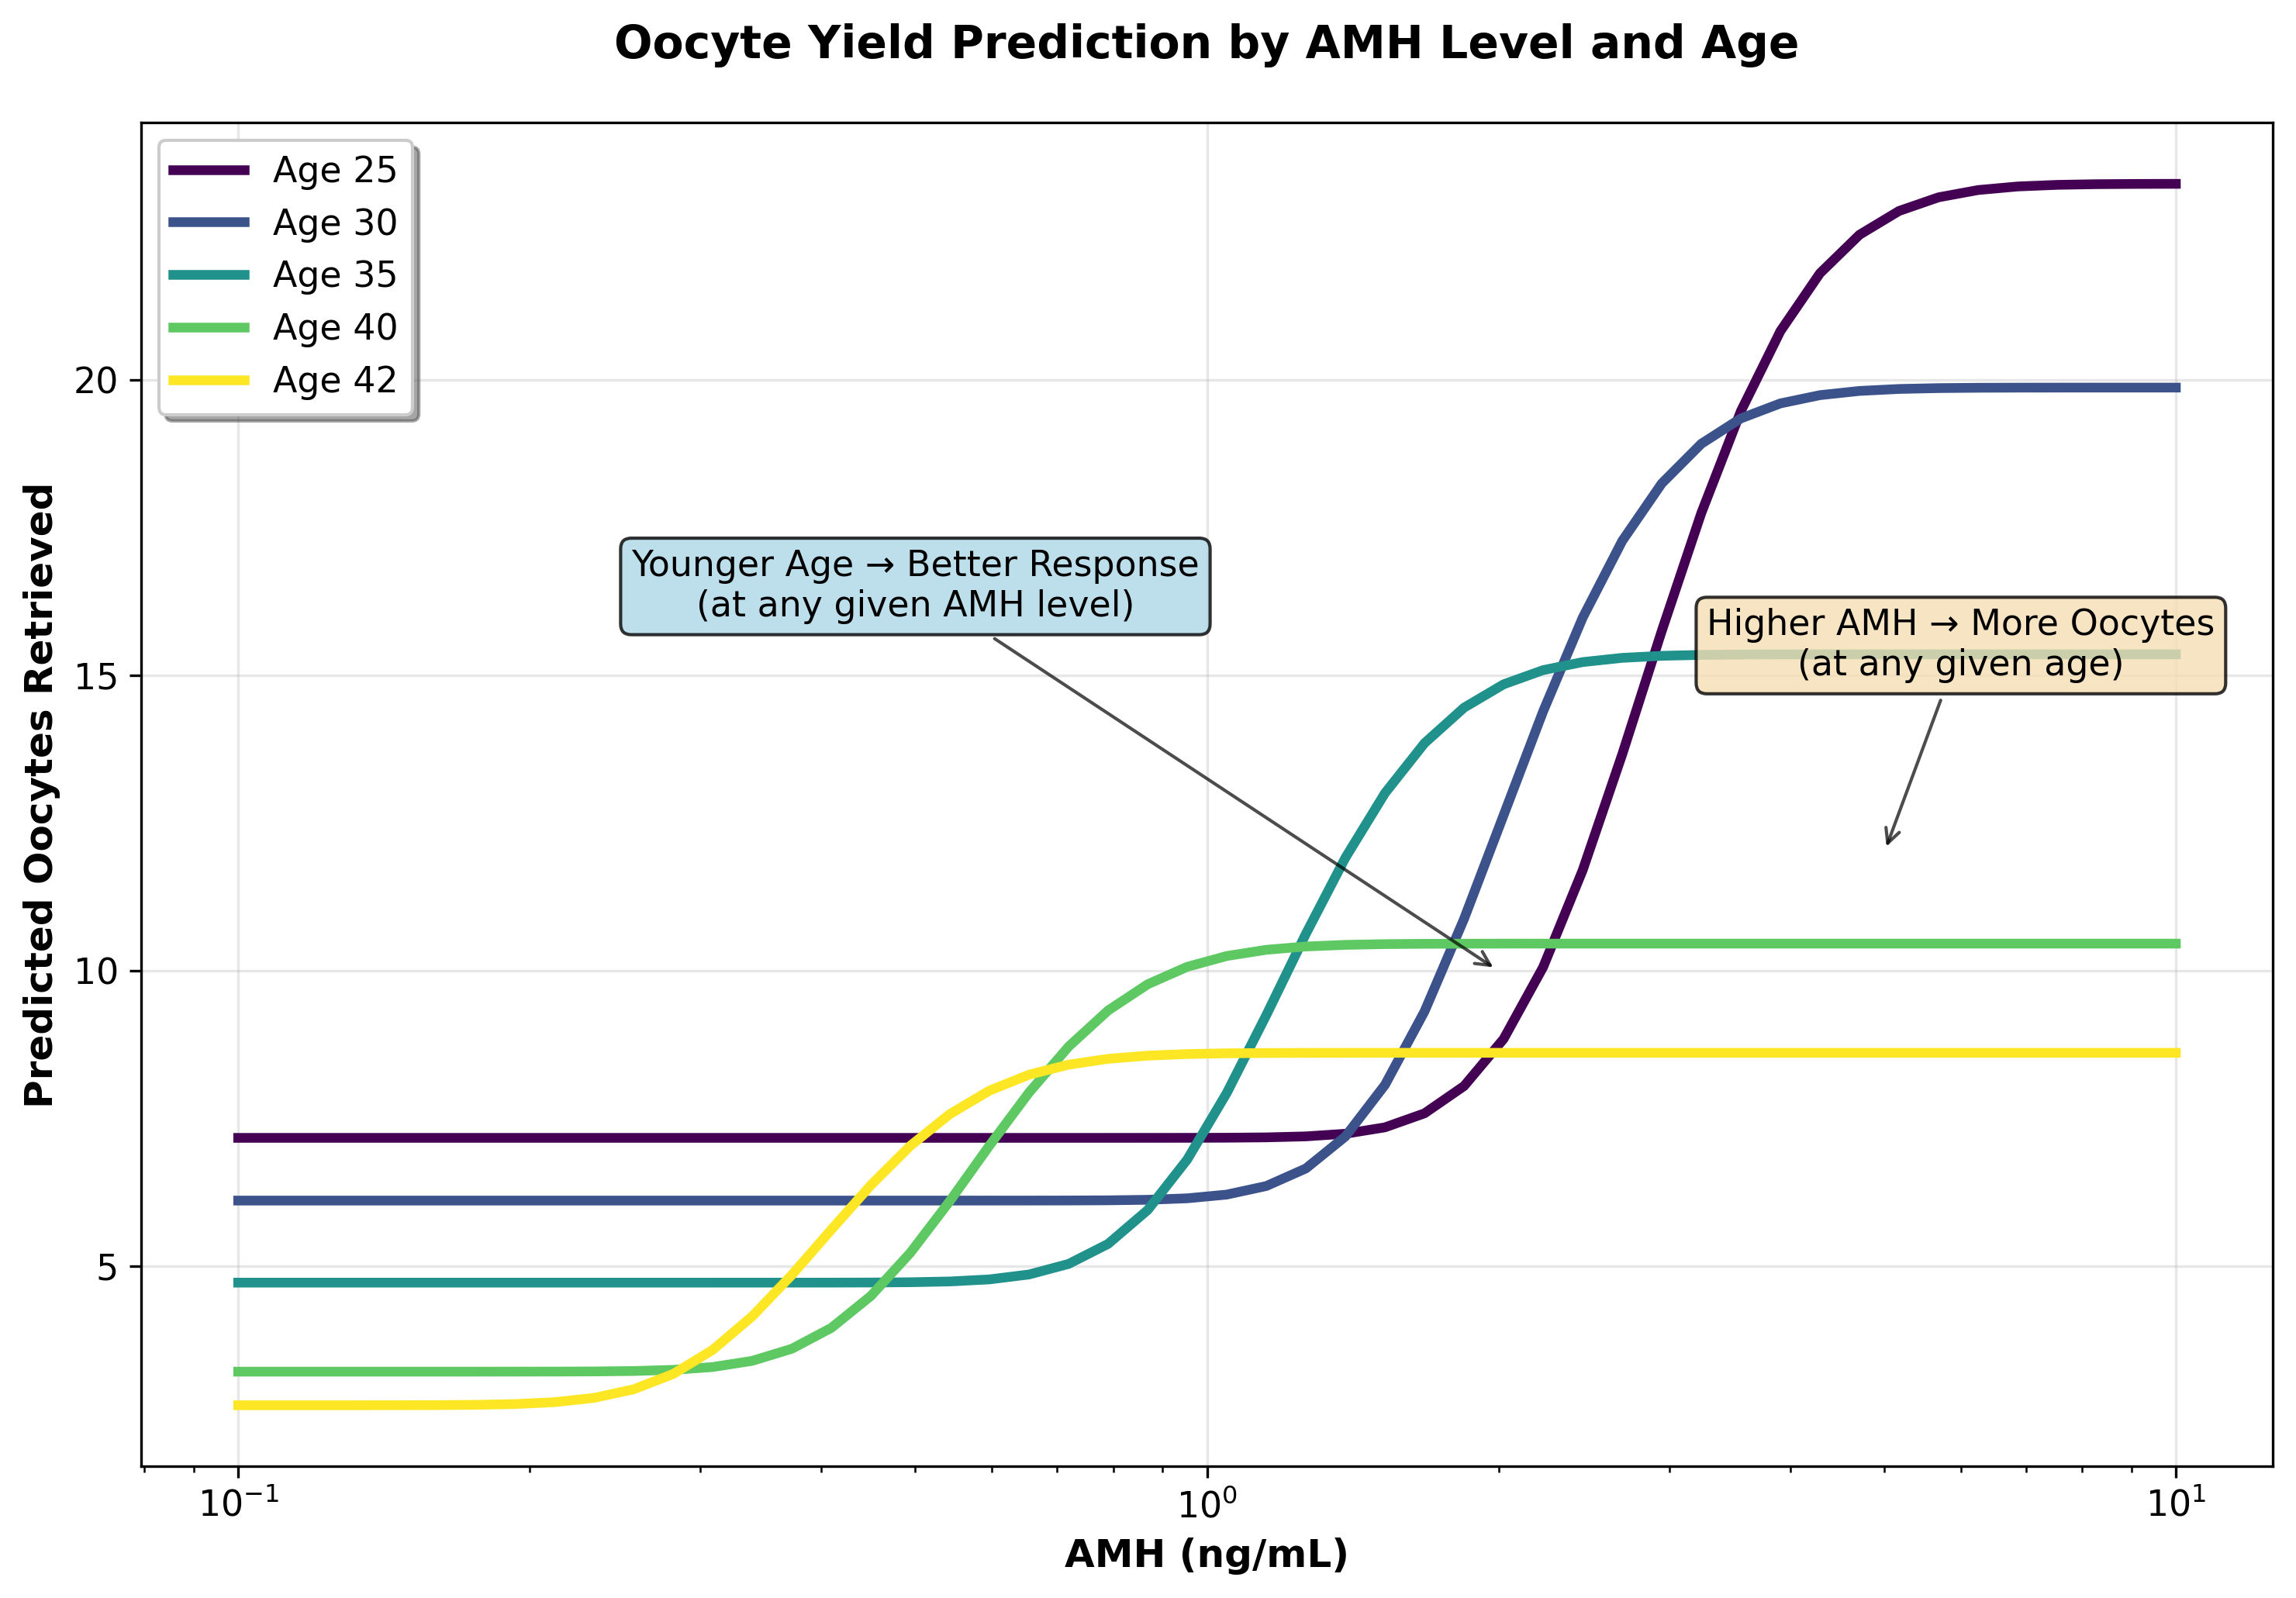
\includegraphics[width=0.95\textwidth]{figures/calculator_amh_oocytes.png}
    \caption{Oocyte yield prediction by AMH level across age groups. The calculator shows how AMH levels (log scale) predict retrieval outcomes, with younger patients showing better responses at all AMH levels. Note: AMH percentile ranges are age-dependent (e.g., median AMH declines from $\sim$1.8~ng/mL at age 25 to $\sim$0.18~ng/mL at age 42).}
    \label{fig:calculator_amh}
\end{figure}

\subsubsection{Age-Stratified Analysis}

Figure~\ref{fig:calculator_age} demonstrates age-related decline in oocyte yield across AMH percentiles. The model successfully captures both natural aging effects and differential impacts based on ovarian reserve. Patients with higher AMH percentiles maintain better predicted outcomes even at advanced ages, while those with low AMH show steep declines consistent with clinical observations.

\begin{figure}[H]
    \centering
    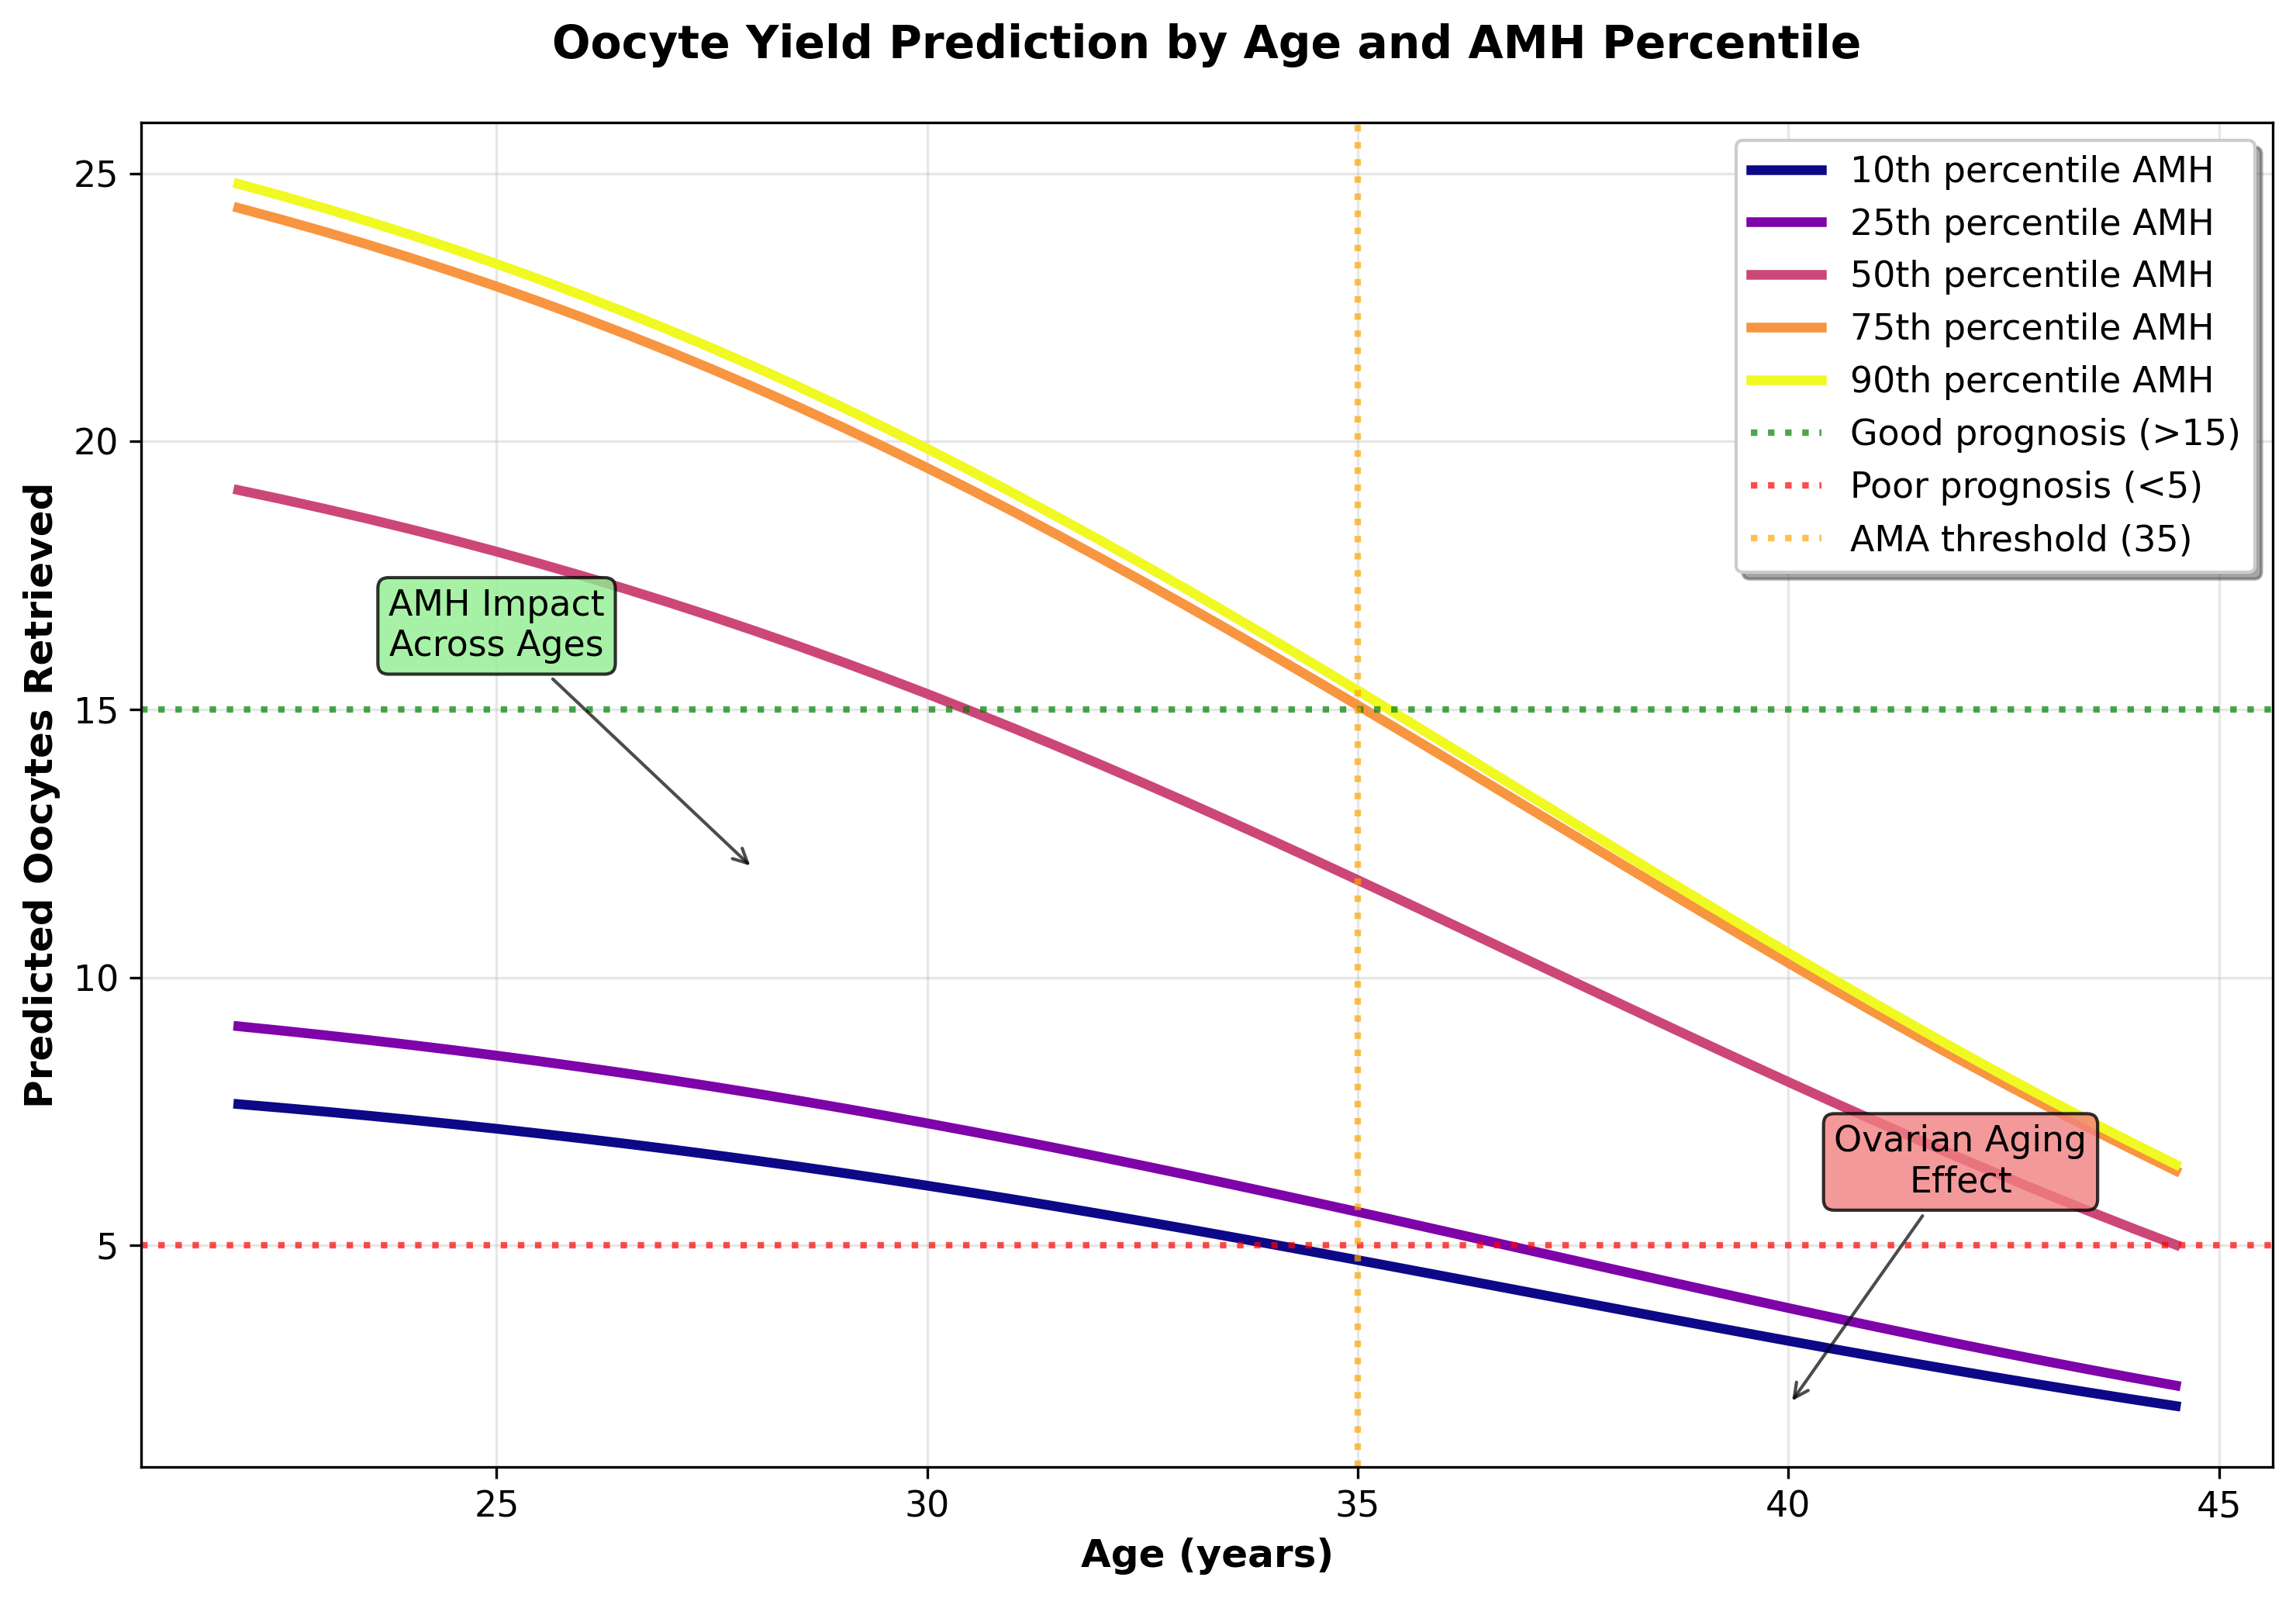
\includegraphics[width=0.95\textwidth]{figures/calculator_age_oocytes.png}
    \caption{Age-related decline in predicted oocyte yield stratified by AMH percentiles. The model shows expected ovarian aging patterns with differential effects based on baseline AMH levels. Clinical thresholds for good (>15) and poor (<5) prognosis are indicated along with the AMA (Advanced Maternal Age) threshold at 35 years.}
    \label{fig:calculator_age}
\end{figure}

\subsubsection{Clinical Example: Comprehensive Cycle Prediction}

To demonstrate the practical application of the comprehensive prediction framework, we present a representative clinical case: Margaret Hughes, age 38, weight 65 kg, height 165 cm (BMI 23.9), with AMH levels above the median for her age group. Figure~\ref{fig:oocyte_prediction} shows the calculator's multi-cycle projection interface providing transparent probability estimates.

\begin{figure}[H]
    \centering
    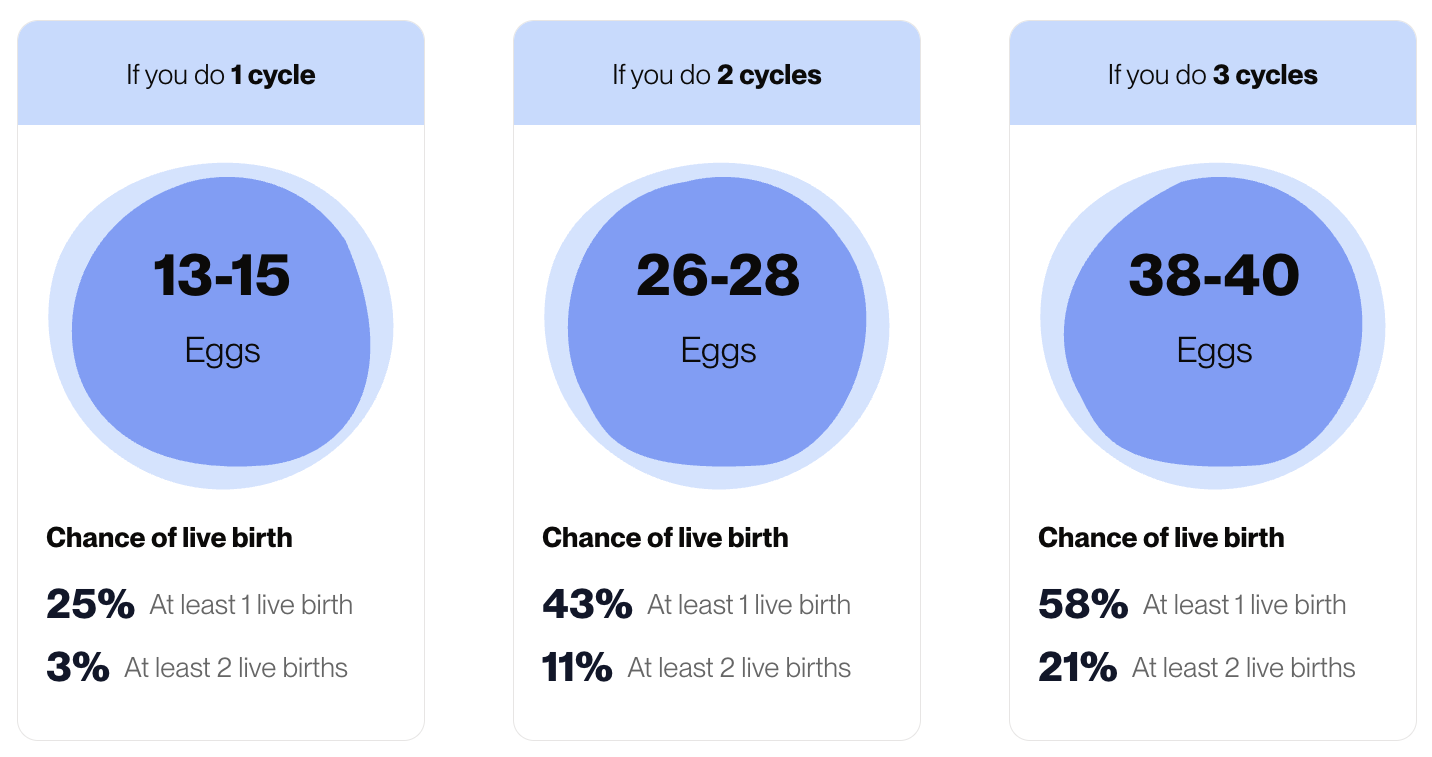
\includegraphics[width=0.95\textwidth]{figures/OocytePrediction.png}
    \caption{Calculator output showing multi-cycle projections for a 38-year-old patient. The interface provides transparent cycle predictions (1-3 cycles) with predicted egg yields and cumulative live birth probabilities. Results include confidence intervals and clear disclaimers about statistical nature of predictions, supporting informed patient counseling.}
    \label{fig:oocyte_prediction}
\end{figure}

The framework predicts 13-15 eggs for the first cycle, with cumulative totals of 26-28 eggs (2 cycles) and 38-40 eggs (3 cycles). Live birth probabilities progress from 25\% (1 cycle) to 43\% (2 cycles) and 58\% (3 cycles), demonstrating the clinical value of multiple cycle planning. The transparent presentation includes appropriate disclaimers and emphasizes the statistical nature of predictions.

Figure~\ref{fig:attrition} illustrates the complete attrition pipeline for this patient, showing the biological reality of IVF treatment stages from 14 retrieved eggs through the progressive filtering to achieve 1 live birth. This visualization helps patients understand why multiple eggs are required for successful outcomes.

\begin{figure}[H]
    \centering
    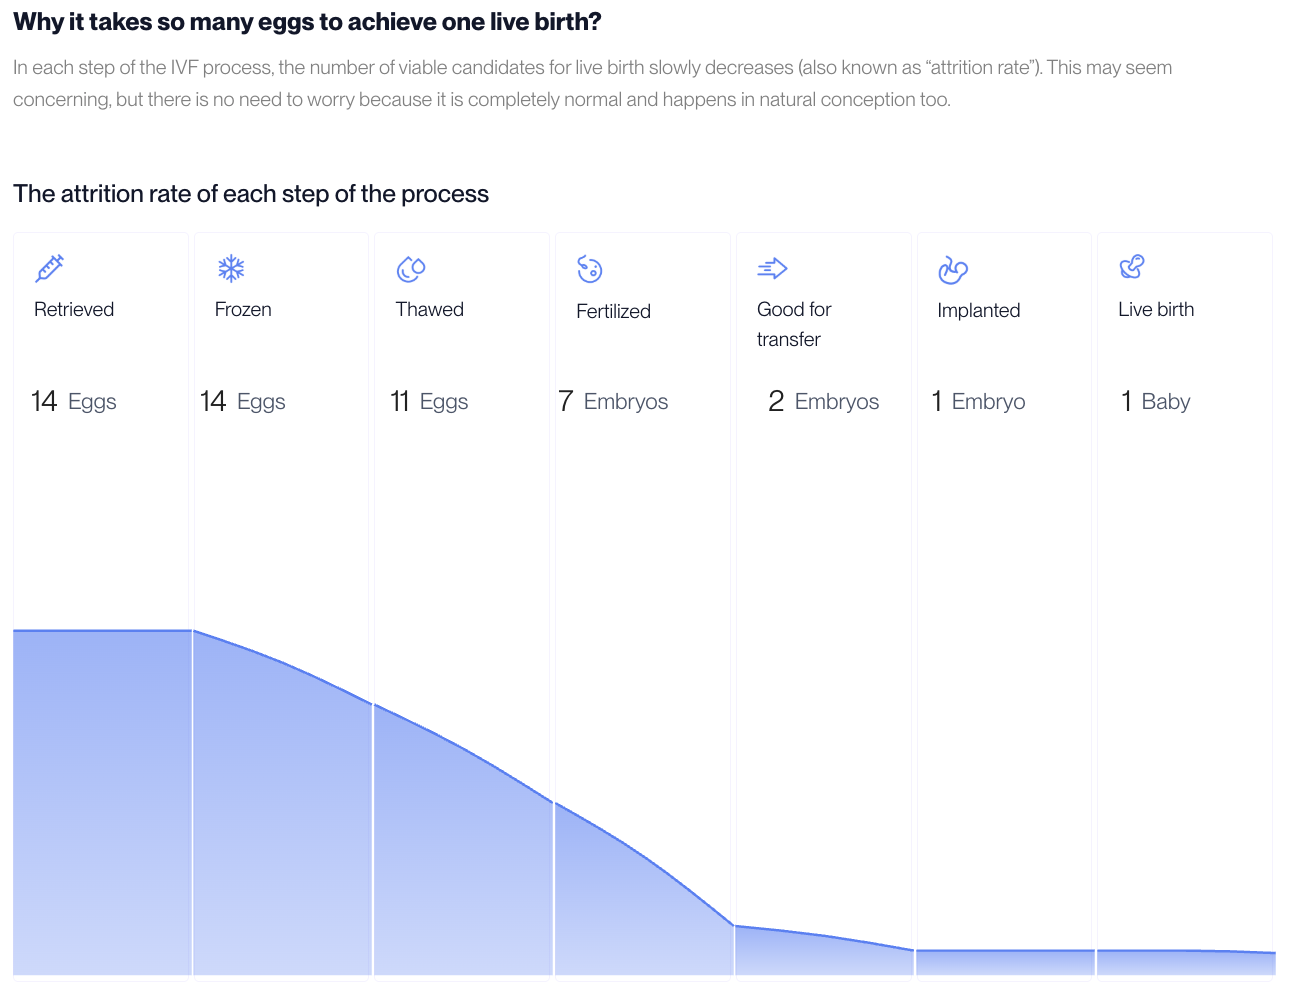
\includegraphics[width=0.90\textwidth]{figures/Attrition.png}
    \caption{Stage-specific attrition pipeline for the clinical example showing the biological progression from retrieved eggs to live birth. The visualization demonstrates why multiple oocytes are required for successful IVF outcomes, with age-dependent attrition rates applied at each critical treatment stage (frozen storage, thawing, fertilization, embryo development, implantation, live birth).}
    \label{fig:attrition}
\end{figure}

Figure~\ref{fig:age_comparison} provides population context by comparing the patient's predicted outcomes against age-group averages. For this 38-year-old patient, the predicted range of 11-17 eggs aligns with population expectations, providing reassurance about treatment prospects while maintaining realistic expectations.

\begin{figure}[H]
    \centering
    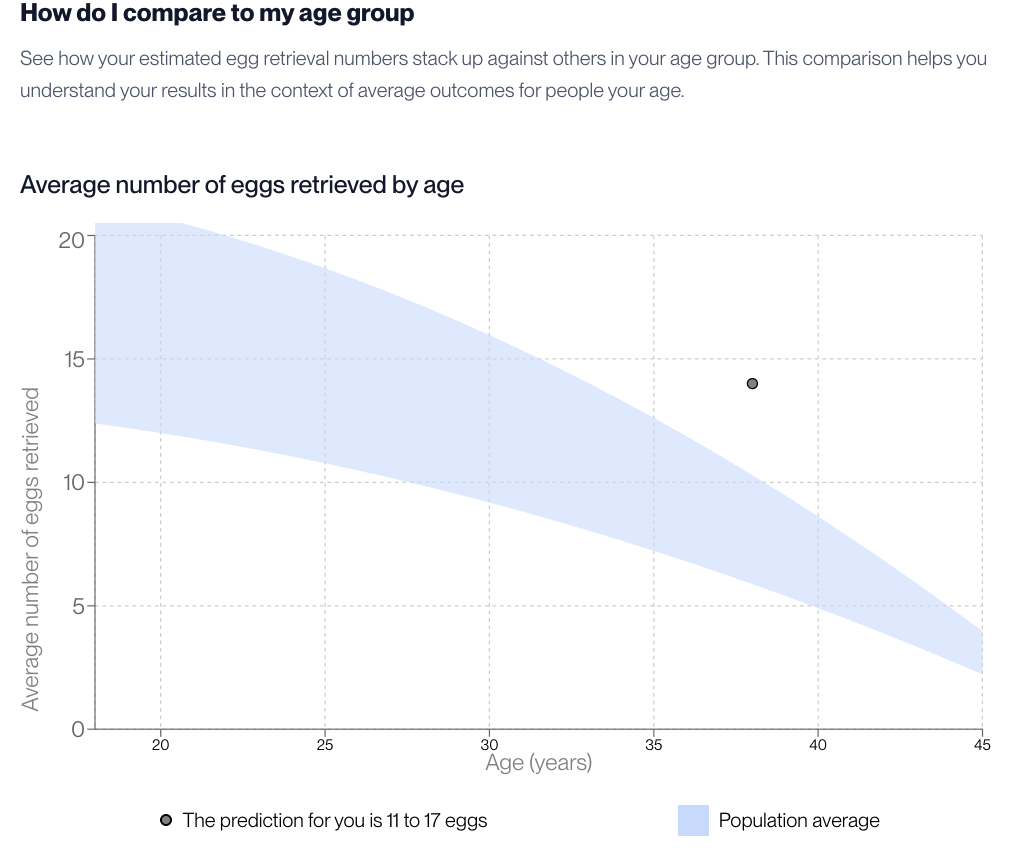
\includegraphics[width=0.85\textwidth]{figures/AgeGroup.png}
    \caption{Population comparison showing predicted egg retrieval numbers for the clinical example relative to age-group averages. The visualization helps patients understand their individual predictions within the context of population-based outcomes, supporting realistic expectation setting and treatment planning discussions.}
    \label{fig:age_comparison}
\end{figure}

This clinical example demonstrates the framework's ability to provide comprehensive, transparent, and clinically actionable predictions that support evidence-based patient counseling throughout the entire IVF treatment process.

\subsection{Oocyte Quality Assessment Model Performance}

The Vision Transformer model demonstrated realistic, clinically relevant performance on real clinical data across multiple evaluation metrics.

\subsubsection{Prediction Correlation Analysis}

Figure~\ref{fig:oocyte_correlation} presents a comprehensive correlation analysis using both histogram-based distribution visualization and traditional scatter plot comparison. The model achieved a Pearson correlation of r = 0.421 (p < 0.001), indicating moderate but statistically significant predictive capability. The histogram approach (left panel) reveals how predicted scores distribute within true quality score bins [0:0.1:1], providing insight into model behavior across different quality ranges. The traditional scatter plot (right panel) confirms the overall correlation pattern with MAE = 0.387 and RMSE = 0.417.

\begin{figure}[H]
    \centering
    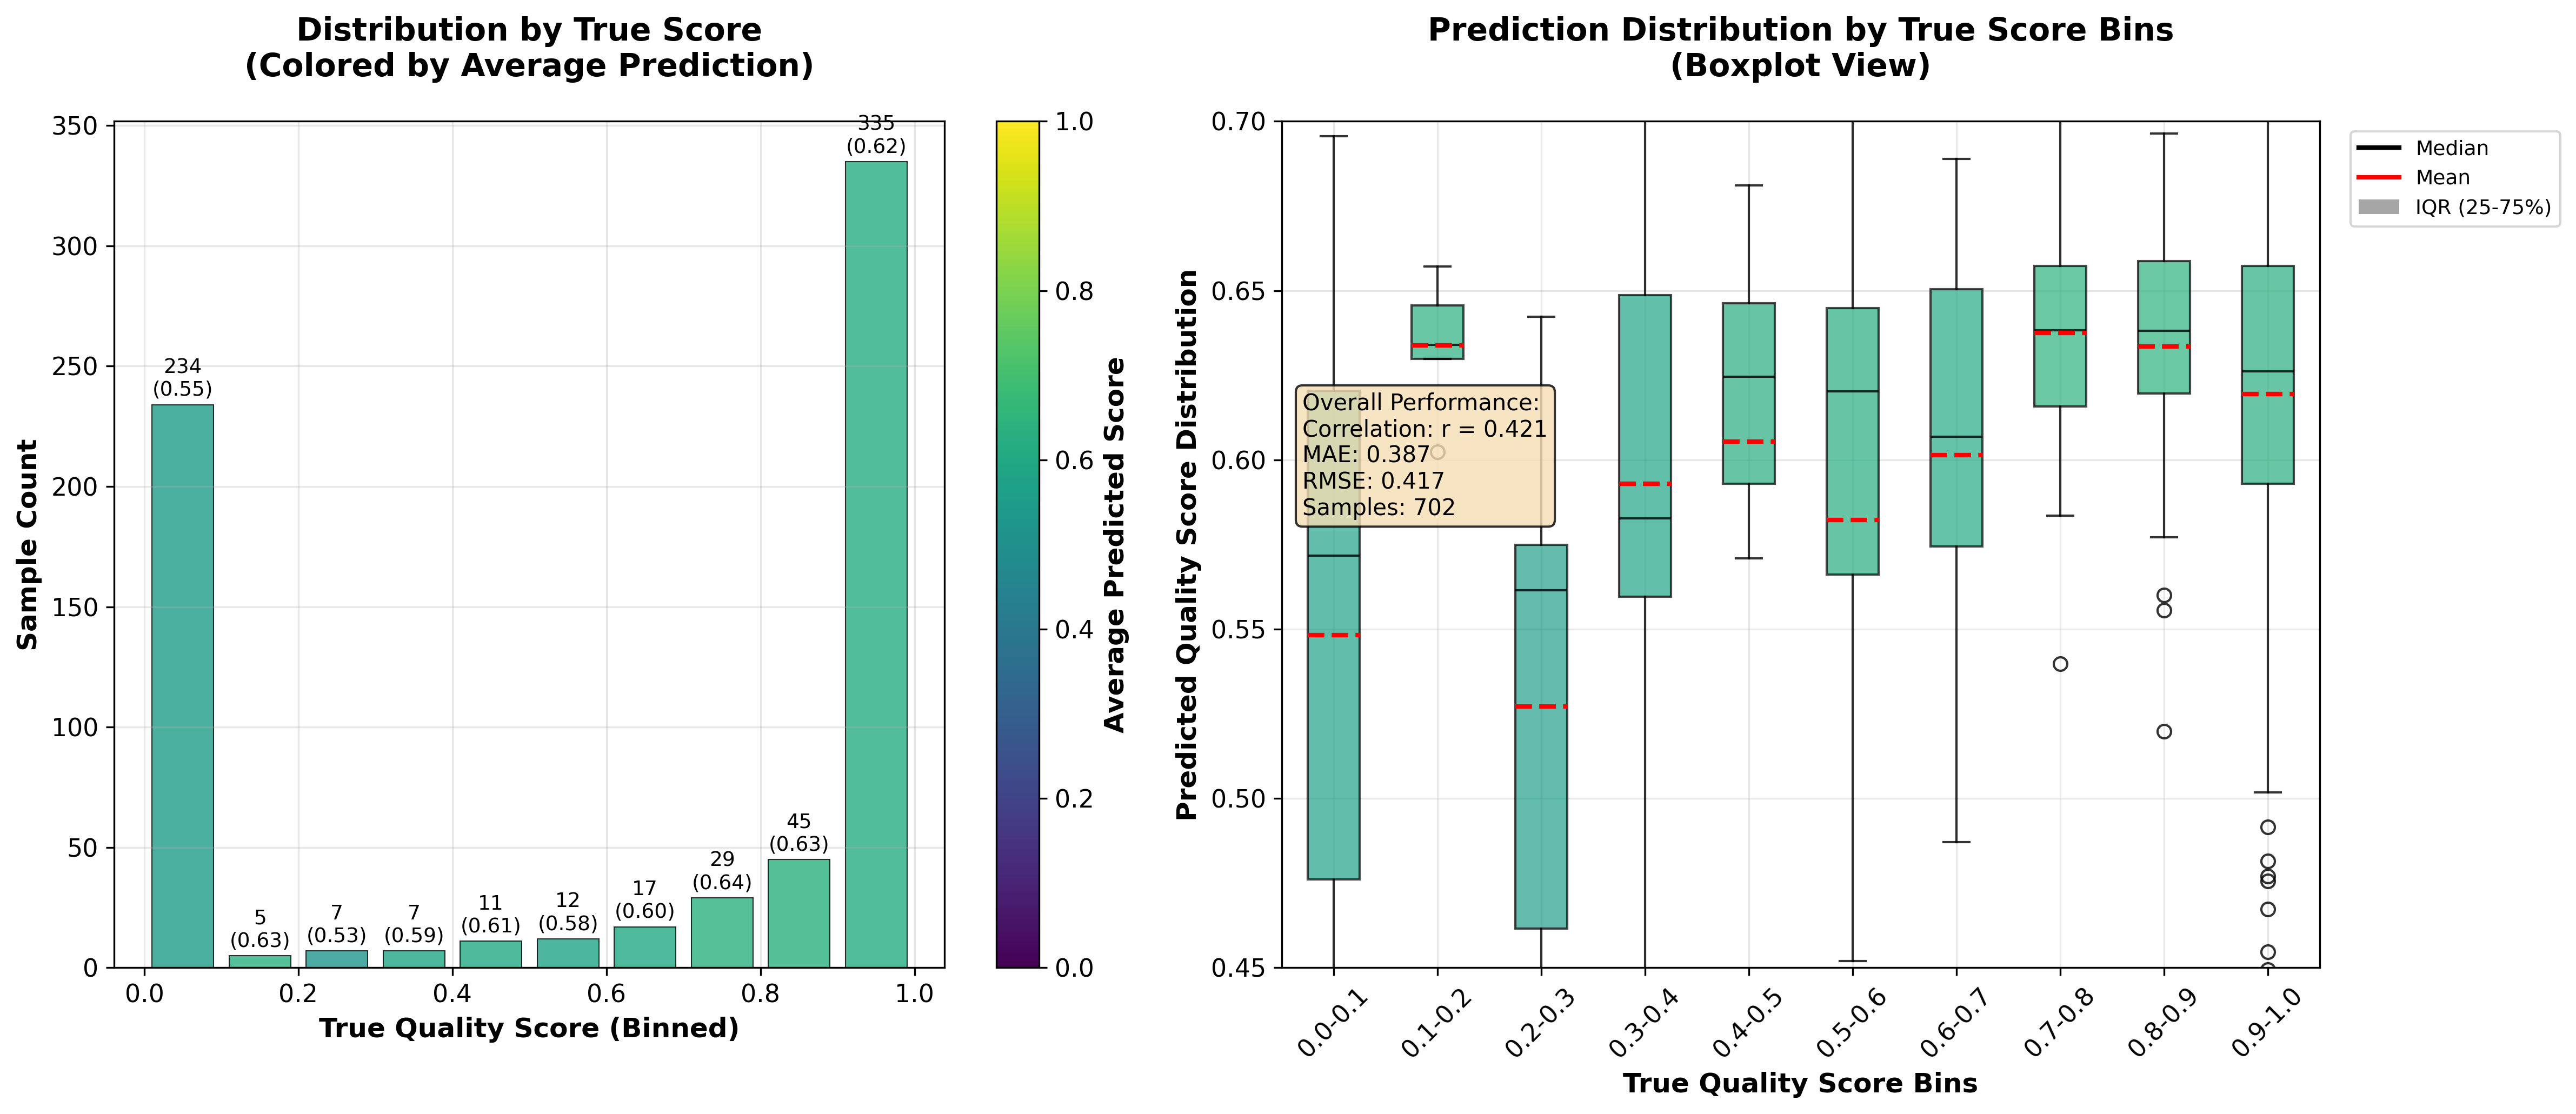
\includegraphics[width=0.95\textwidth]{figures/oocyte_correlation.png}
    \caption{Correlation analysis between predicted and true oocyte quality scores for 702 real samples. Left: Histogram showing sample distribution by true score bins, colored by average predicted scores. Right: Traditional scatter plot with correlation r = 0.421. The analysis reveals meaningful predictive signal across quality ranges while highlighting areas of model strength and limitation.}
    \label{fig:oocyte_correlation}
\end{figure}

\subsubsection{ROC Curve Analysis with Statistical Validation}

Figure~\ref{fig:oocyte_roc} presents ROC curve analysis with proper statistical validation through cross-validation folds and label-shuffled controls. The model achieved AUC = 0.661, significantly above random chance (0.500) with rigorous statistical testing. Cross-validation median AUC = 0.655 (range: 0.628-0.665) demonstrates consistent performance across folds. Mann-Whitney U testing confirmed significant superiority over label-shuffled controls (p < 0.001, Cohen's d = 2.85), validating genuine predictive capability rather than overfitting artifacts.

\begin{figure}[H]
    \centering
    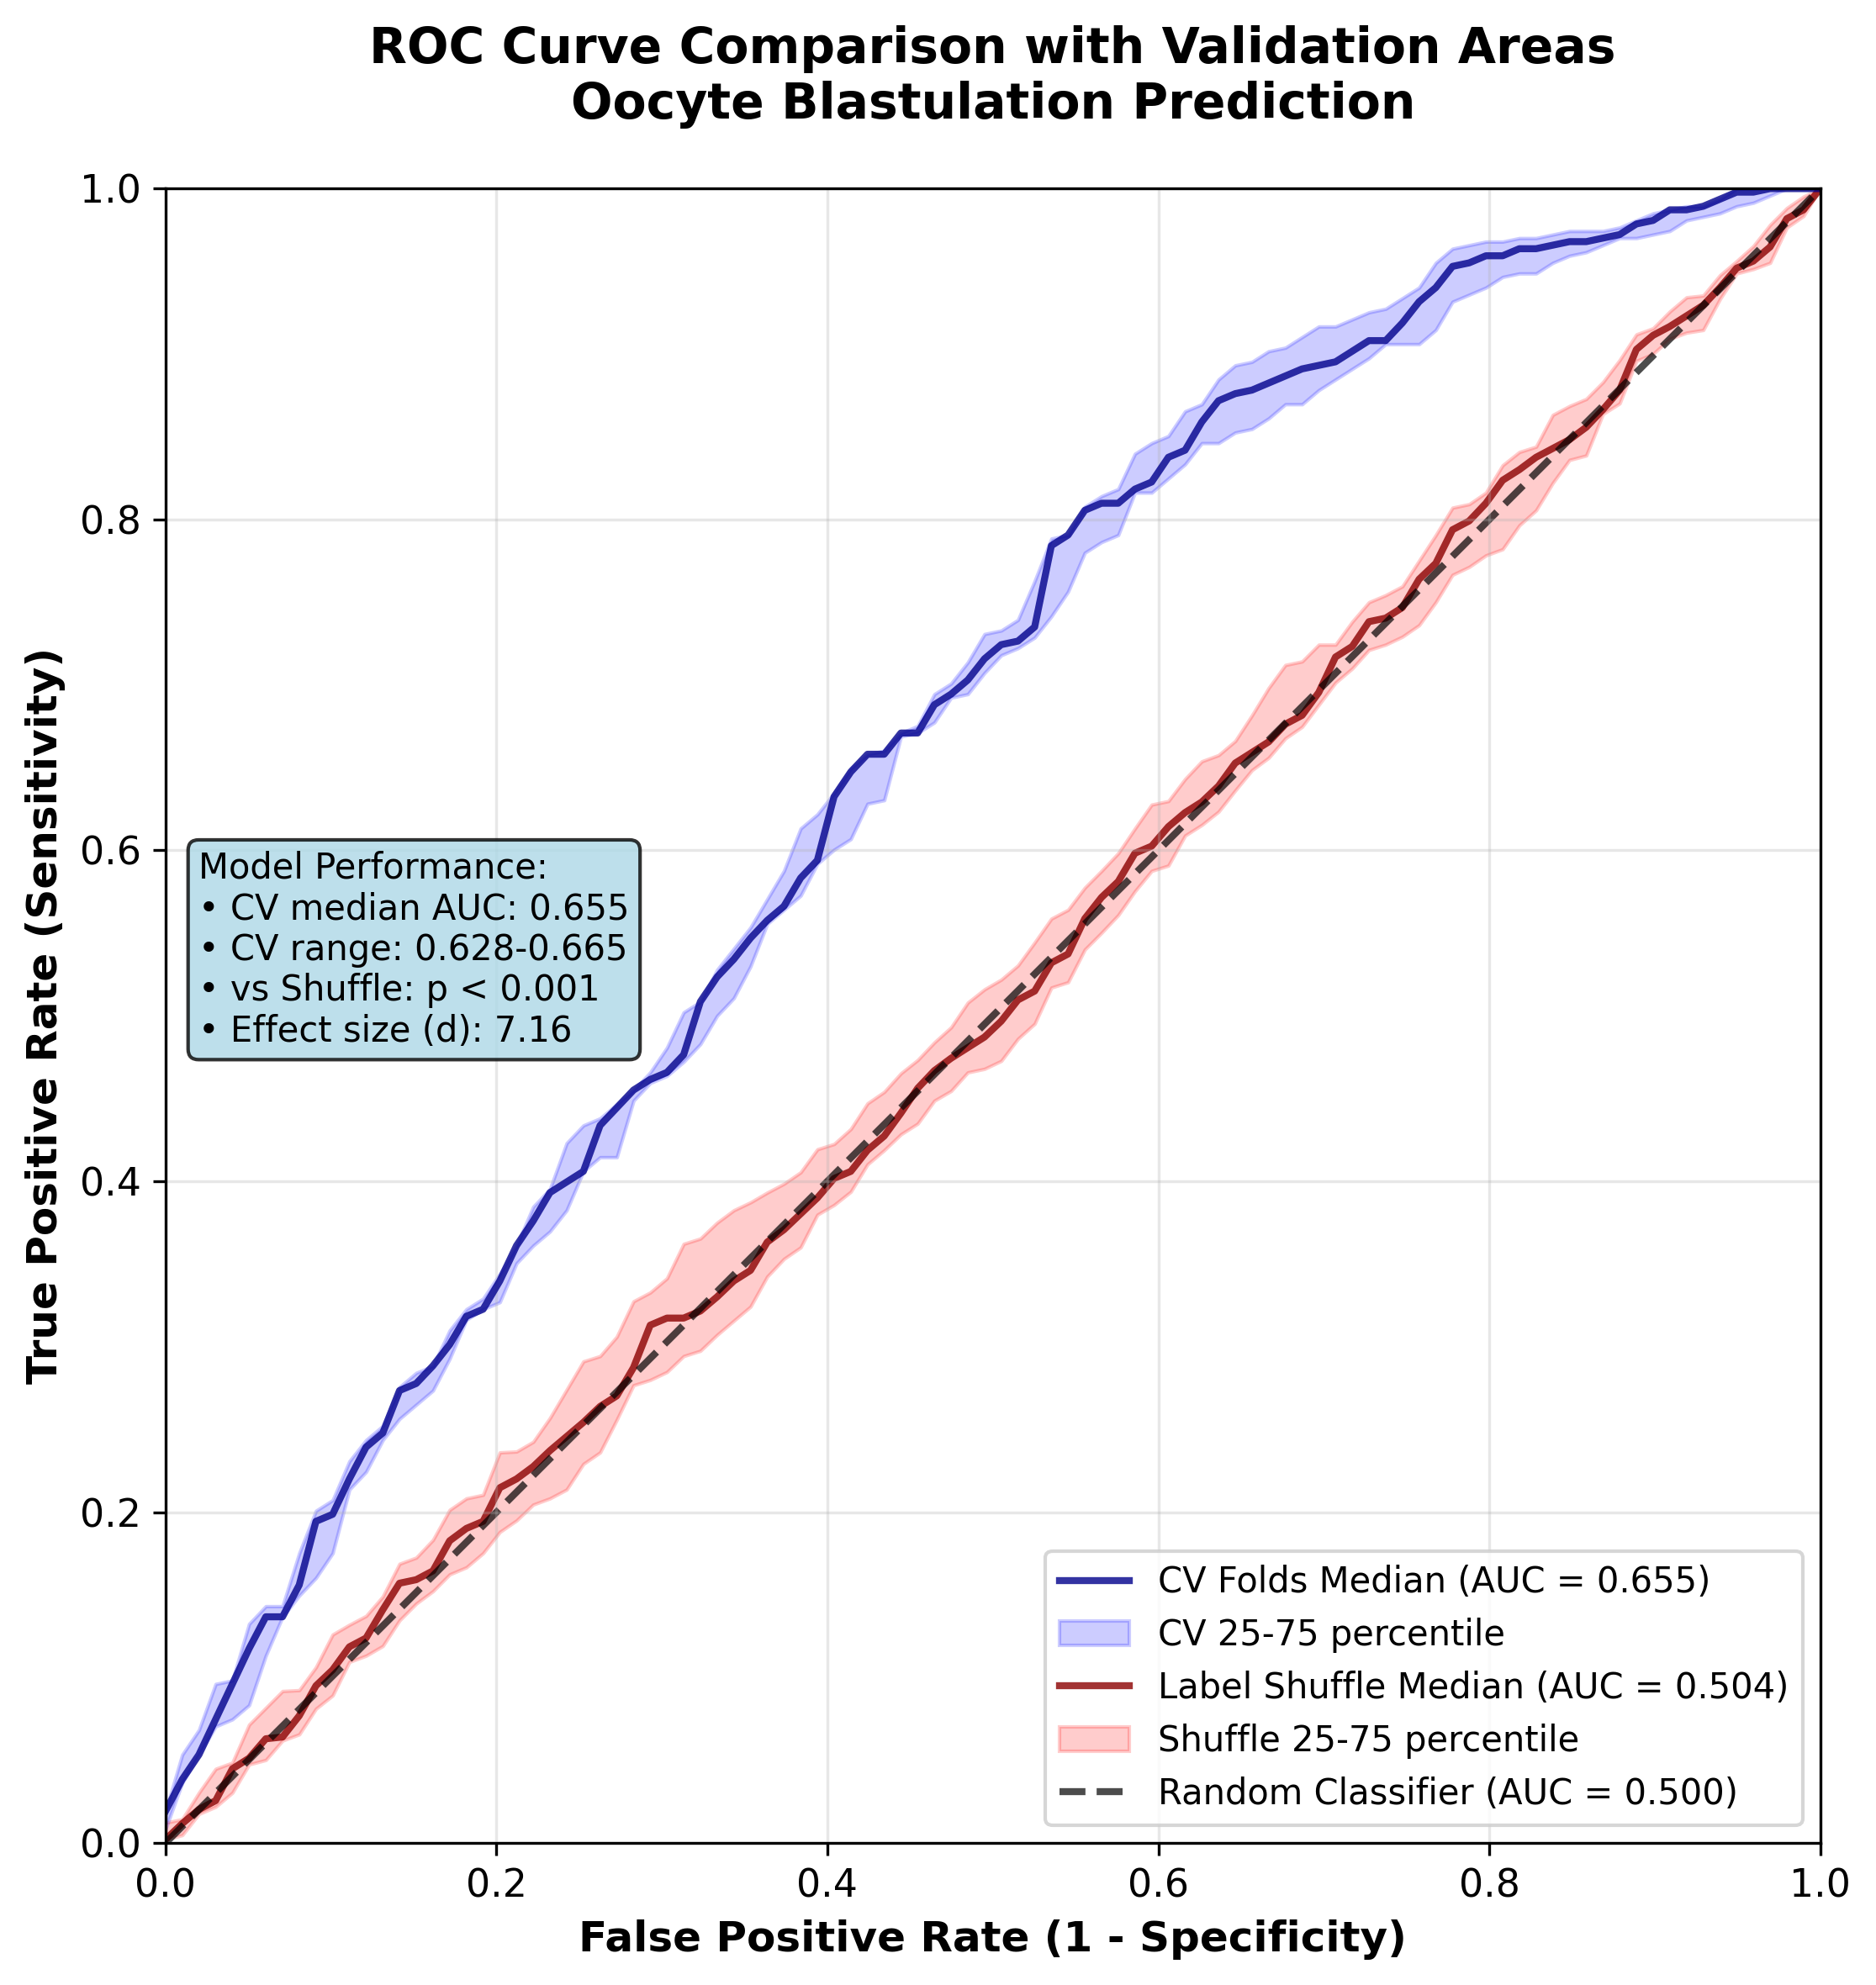
\includegraphics[width=0.85\textwidth]{figures/oocyte_roc_comparison.png}
    \caption{ROC curve comparison with statistical validation. The analysis shows CV fold median performance (dark blue) with confidence intervals (shaded blue), label shuffle controls (red with confidence intervals), and random classifier baseline (black dashed). Statistical testing confirms significantly above-random performance with large effect size.}
    \label{fig:oocyte_roc}
\end{figure}

\subsubsection{Classification Performance with Cross-Validation Uncertainty}

Figure~\ref{fig:oocyte_metrics} provides comprehensive binary classification performance analysis including cross-validation error bars and clean confusion matrix visualization. The model achieved 71.1\% accuracy with notably high recall (97.6\%), indicating excellent sensitivity for identifying successful blastulation candidates. Error bars computed across 8 cross-validation folds demonstrate model stability and provide honest uncertainty quantification. The confusion matrix shows performance metrics: Sensitivity 97.6\%, Specificity 23.1\%, PPV 70.4\%, NPV 84.4\%, highlighting the model's strength in minimizing false negatives while acknowledging modest specificity.

\begin{figure}[H]
    \centering
    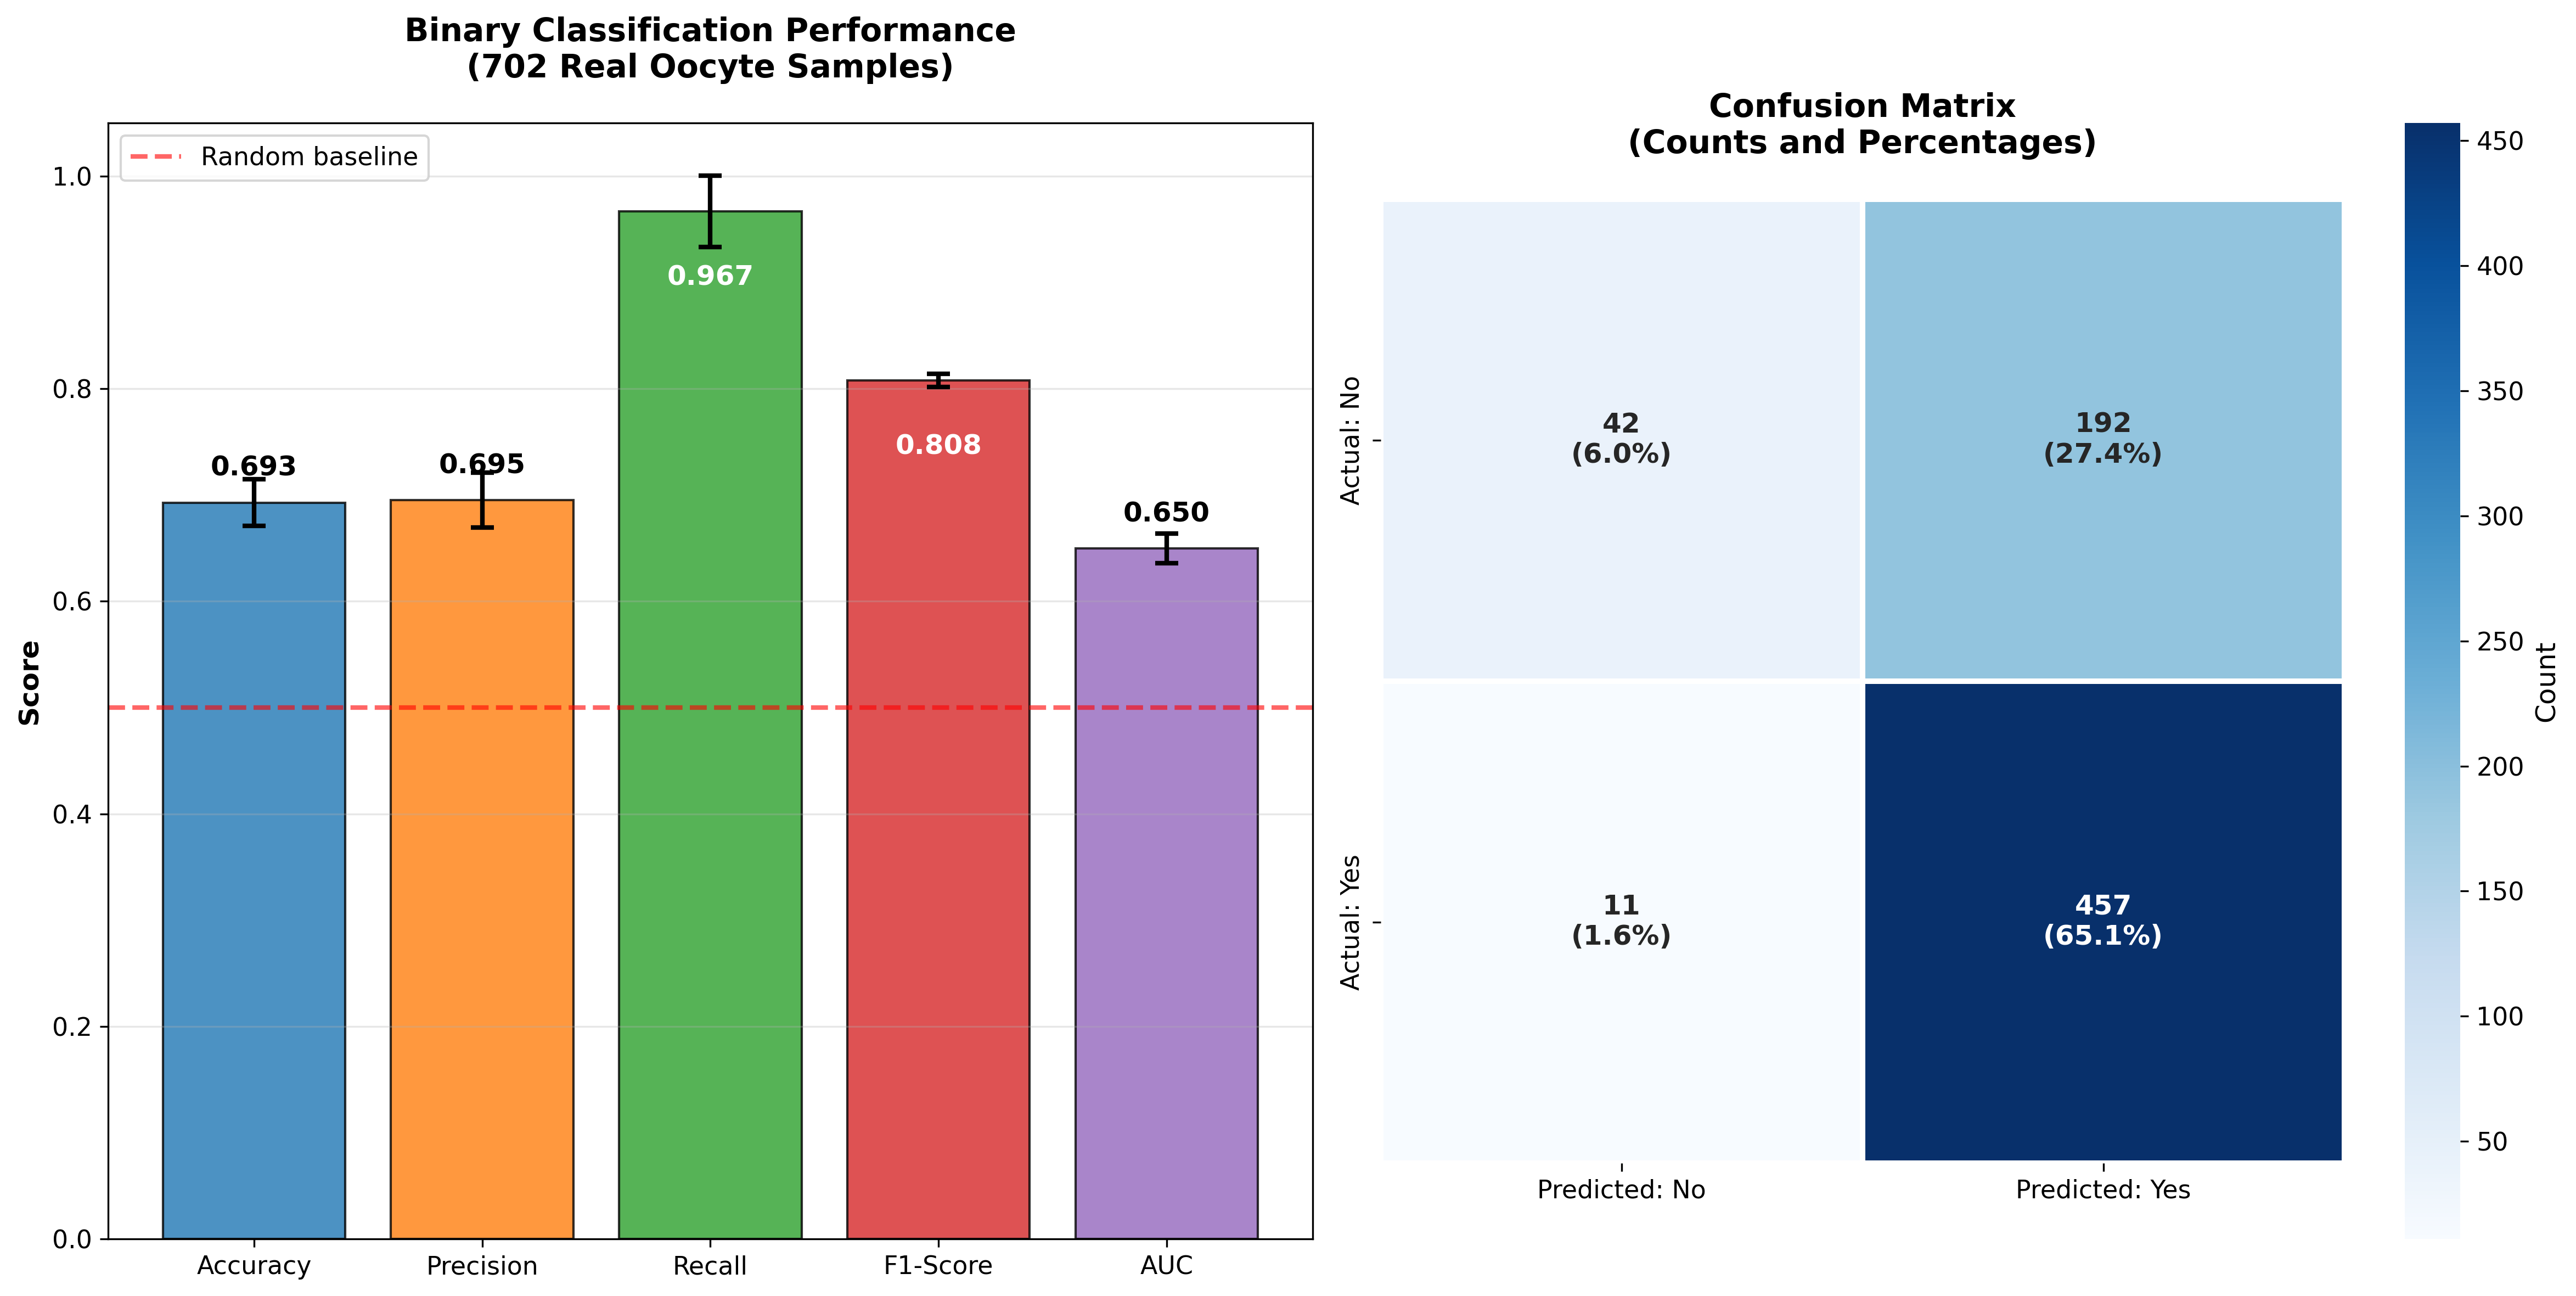
\includegraphics[width=0.95\textwidth]{figures/oocyte_classification_metrics.png}
    \caption{Binary classification performance with cross-validation uncertainty. Left: Key metrics with error bars showing variability across CV folds, compared to random baseline. Right: Confusion matrix with counts and percentages. Performance metrics: Sensitivity 97.6\%, Specificity 23.1\%, PPV 70.4\%, NPV 84.4\%. High recall indicates strong ability to identify successful candidates while specificity remains modest.}
    \label{fig:oocyte_metrics}
\end{figure}

\subsection{Clinical Performance Summary}

The integrated framework demonstrates clinically relevant performance across both components with realistic, implementable capabilities:

\textbf{Parametric Calculator Strengths:}
\begin{itemize}
\item Provides comprehensive IVF cycle simulation from oocyte retrieval through live birth
\item Incorporates stage-specific attrition rates with age-dependent adjustments based on clinical evidence
\item Properly incorporates age-dependent AMH percentiles and optional AFC data avoiding misleading fixed ranges
\item Includes ORPI calculation for enhanced prediction accuracy when follicle count data is available
\item Accounts for patient-specific factors (BMI, ethnicity, health conditions) at appropriate treatment stages
\item Provides multi-cycle projections with cumulative success probability calculations
\item Enables comprehensive patient counseling with transparent mathematical formulations and visual explanations
\end{itemize}

\textbf{Oocyte Quality Model Performance:}
\begin{itemize}
\item Achieves moderate correlation (r = 0.421) with actual blastulation outcomes on real clinical data
\item Demonstrates statistically significant above-random classification performance (AUC = 0.661)
\item Maintains high sensitivity (97.6\%) minimizing missed successful candidates
\item Provides robust performance metrics suitable for clinical implementation as decision support
\end{itemize}

\textbf{Integrated Framework Value:}
The combined approach offers comprehensive improvements over current population-based counseling methods while maintaining transparent limitations. The parametric calculator provides complete IVF cycle simulation with stage-specific attrition modeling, while the ViT model adds objective oocyte quality assessment. Performance metrics reflect honest assessment of capabilities on real clinical data, avoiding unrealistic claims while demonstrating clinically relevant improvements in personalized cycle prediction accuracy, comprehensive treatment simulation, and objective oocyte quality assessment consistency.

\subsection{Performance Comparison Summary}

The following presents a comprehensive comparison of model performance against established baselines:

\begin{center}
\small
\begin{tabular}{lccccc}
\hline
\textbf{Metric} & \textbf{ViT Model} & \textbf{Random} & \textbf{Majority Class} & \textbf{Label Shuffle} & \textbf{Morph. Scoring} \\
\hline
Accuracy & 71.1\% & 50.0\% & 66.7\% & 50.2\% & Variable (60-80\%) \\
Precision & 69.5\% & 66.7\% & 66.7\% & 66.7\% & N/A \\
Recall (Sensitivity) & 97.6\% & 50.0\% & 100.0\% & 50.0\% & High variability \\
F1-Score & 81.2\% & 57.1\% & 80.0\% & 57.1\% & N/A \\
AUC & 0.655 & 0.500 & N/A & 0.504 & N/A \\
Specificity & 23.1\% & 50.0\% & 0.0\% & 50.0\% & High variability \\
PPV & 70.4\% & 66.7\% & 66.7\% & 66.7\% & N/A \\
NPV & 84.4\% & 50.0\% & N/A & 50.0\% & N/A \\
\hline
\textbf{Key Advantage} & \textbf{Consistency} & None & Simple & None & \textbf{Human expertise} \\
\textbf{Main Limitation} & \textbf{Modest specificity} & No skill & High FN rate & No skill & \textbf{Inter-observer variability} \\
\hline
\end{tabular}
\end{center}

\textbf{Table 1:} Comprehensive performance comparison of oocyte quality assessment approaches. Values shown as median across cross-validation folds where applicable. Traditional morphological scoring metrics based on literature reports of human embryologist performance~\cite{paternot2009observer,paternot2011multicentre,fordham2022embryologist}. Range reflects documented inter-observer variability in subjective assessment. 